\section{Experimental Results}
This section will show and compare results obtained from original approaches, our implementation of them and their adoption to federated learning. As mentioned in section \ref{sec:dev_and_training} we did not want to change more than absolutely necessary from the original implementation, including the testing and evaluation methods, which is why the presentation and form of results can differ from one paper to another. All federated training results are gained with a 4 client setup.


\subsection{Federation Paper}\label{subsec:results_federation_paper}
For the \textit{federation paper} we did the most tests as we used it continuously during the project phase to improve our understanding and our implementation of the automated federation test. Table \ref{tab:results_federation_paper} shows the accuracy values obtained from different runs.

\begin{table}[htbp]
    \small
    \centering
    \caption{Comparison between federation paper\cite{federated_machine_learning} and our ResNet implementation.}
    \begin{tabular}{c|c|c|c|c}
        Model & Optimizer & \shortstack[c]{Data\\distribution} & Avg. method & Accuracy\\
        \hline
        FedPaper (cent.) & SGD & - & - & 0.9734 \\
        FedPaper (cent.) & Adam & - & - & 0.9664 \\
        FedPaper (fed.) & SGD & Duplicate & FedSGD & 0.9872\\
        FedPaper (fed.) & Adam & Duplicate & FedSGD & 0.9828\\
        ResNet (cent.) & Adam & - & - & 0.9649 \\
        ResNet (fed.) & Adam & Duplicate & FedSGD & 0.9886 \\
        ResNet (fed.) & Adam & Split & FedSGD & 0.9764 \\
        ResNet (fed.) & Adam & Split \& Augment & FedSGD & 0.9230 \\
        ResNet (fed.) & Adam & Split & FedAvg & 0.9596 \\
    \end{tabular}
    \label{tab:results_federation_paper}
\end{table}

The first four entries are taken from the paper itself and represent the baseline performance we wanted to match. As can be seen, our centralized learning implementation (row 5) has an accuracy less than 1\% worse than the best centralized value from the paper. 
The next row, which shows our federated ResNet with duplicated data on each client confirms the authors claim that the federation algorithm performs even better than the centralized one.
In real world scenarios the data is never duplicated on each client device, as this would defeat the purpose of federated learning.
This is why we also tested our implementation with an evenly, randomly split dataset on each client (row 7), which does not perform as good as the previous test but still better than the centralized model.
Row 8 shows the same test but with data that was additionally augmented to make the images less similar with each other. Curiously, this results in the worst performance of all runs. One explanation for this is that the model simply needs more epochs of training to learn the added variation in the data. Another explanation is that, because testing of this model was still done with un-augmented data, the results of the other models show some form of over-fitting to the given images which is not apparent in the current model.
The last row repeats the experiment from row 7, but uses Federated Averaging with 5 local epochs on each client for each global epoch instead of Federated SGD to aggregate the client model parameters. In theory this should perform better than its Federated SGD counterpart.

\subsection{COVID-Net}
The COVID-Net implementation from the authors had its own result metrics evaluation using sensitivity, specificity, positive predictive value and negative predictive value, the corresponding values can be seen in table \ref{tab:results_covidnet}. 

\begin{table}[htbp]
    \captionsetup[table]{justification=centering}
    \small
    \centering
    \caption{Comparison between COVID-Net paper\cite{covid_net} and our training of it.}
    \begin{tabular}{c|c|c|c|c}
        Model & Sensitivity & Specificity & \shortstack[c]{Positive\\predictive value}  & \shortstack[c]{Negative\\predictive value}\\
        \hline
        Original & 0.955 & 0.970 & 0.970 & 0.956 \\
        Our training (cent.) & 0.995 & 0.430 & 0.636 & 0.989 \\
        Our training (fed.) & - & - & - & -\\
    \end{tabular}
    \label{tab:results_covidnet}
\end{table}

As described in section \ref{subsec:dev_covidnet}, re-training of this model was not successful. Both specificity and positive predictive value are a lot worse than with the available pre-trained model. We did not attempt to implement a federated learning version because the results would not have been representative anyway if our centralized results are not at least close to the ones given by the authors.

\subsection{DLH-COVID}
The results for the DLH-COVID model depicted in table \ref{tab:results_dlh_covid} show that, with our centralized training, we could not quite match the metric scores taken from the paper, but our federated learning approach still performed better than the centralized one in every regard and is not that far off from the original results.

\begin{table}[htbp]
    \small
    \centering
    \caption{Comparison between DLH-COVID paper\cite{dlh_net} and our training of it.}
    \begin{tabular}{c|c|c|c|c}
        Model & Accuracy & Precision & Recall & F1-Score \\
        \hline
        Original & 0.967 & 0.965 & 0.958 & 0.961 \\
        Our training (cent.) & 0.947 & 0.950 & 0.928 & 0.939\\
        Our training (fed.) & 0.950 & 0.952 & 0.934 & 0.942\\
    \end{tabular}
    \label{tab:results_dlh_covid}
\end{table}

Additionally to the accuracy, precision, recall and f1-score the authors of the DLH-COVID paper also included a visual result evaluation in form of a heatmap, which can be seen in figure \ref{fig:dlh_all_heatmaps}.

\begin{figure}[htbp]
    \captionsetup[subfigure]{justification=centering}
    \centering
    \begin{subfigure}{.35\textwidth}
        \centering
        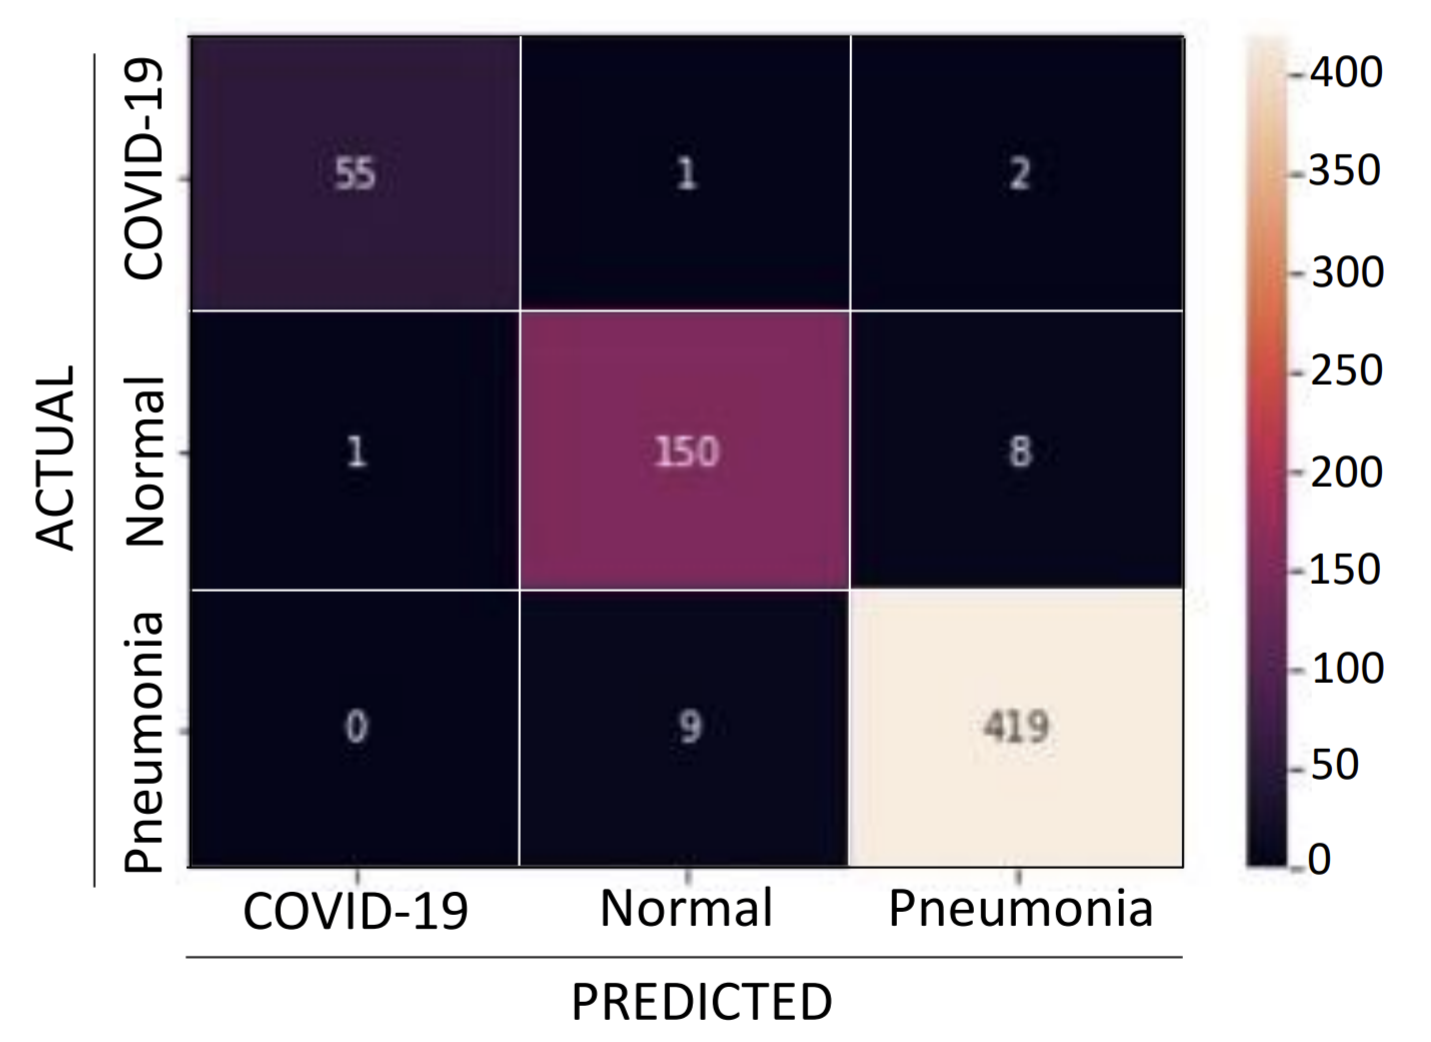
\includegraphics[width=\linewidth]{imgs/dlh_covid_paper_heatmap.png}
        \caption{DLH-COVID Paper}
        \label{fig:dlh_original_heatmap}
    \end{subfigure}

    \vspace{.3cm}
    \begin{subfigure}{.35\textwidth}
      \centering
      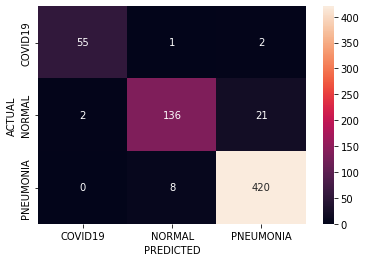
\includegraphics[width=\linewidth]{imgs/dlh_covid_own_seq_heatmap.png}
      \caption{Our DLH-COVID training}
      \label{fig:dlh_seq_heatmap}
    \end{subfigure}
    \begin{subfigure}{.35\textwidth}
      \centering
      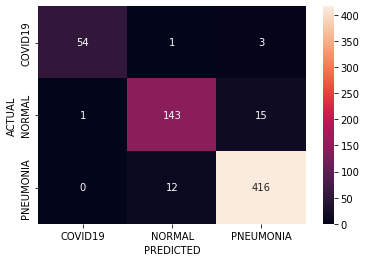
\includegraphics[width=\linewidth]{imgs/dlh_covid_own_fed_heatmap.png}
      \caption{Our federated DLH-COVID training}
      \label{fig:dlh_fed_heatmap}
    \end{subfigure}
    \caption{Heatmap comparison between DLH-COVID paper\cite{dlh_net} and our training of it.}
    \label{fig:dlh_all_heatmaps}
\end{figure}

It shows the absolute values of actual COVID-19, Pneumonia and normal images on the left side and how many of those were predicted in which category on the bottom. Our federated training predicted slightly less disease images correct, but it was more often correct on normales images than the sequentially trained model.

\subsection{DarkCovidNet}
Table \ref{tab:results_darkcovidnet} contains the results for DarkCovidNet. Our training, both centralized and federated, was again not as good as the score reported in the paper. With a 5\% difference between the centralized models, it might be argued that the federated learning score is not really an indication of what a federated version of the authors training process could achieve, but because of the improvements we see in our training we think it could further improve the authors scores. This model is also the first and only one in our research where a federated training process performs worse than the model trained centrally.

\begin{table}[htbp]
    \small
    \centering
    \caption{Comparison between DarkCovidNet paper\cite{dark_net} and our training of it.}
    \begin{tabular}{c|c|c}
        Model & Avg. method & Accuracy (\%)\\
        \hline
        Original & - & 0.870 \\
        Our training (cent.) & - & 0.828\\
        Our training (fed.) & FedSGD & 0.764 \\
        Our training (fed.) & FedAvg & 0.838 \\
    \end{tabular}
    \label{tab:results_darkcovidnet}
\end{table}

In contrast to the results from section \ref{subsec:results_federation_paper} the Federated Averaging really did perform better than the SGD variant, and also better than our centralized model.

\subsection{GraphCovidNet}
The results from GraphCovidNet, which again include precision, recall, f1-score and accuracy and can be seen in table \ref{tab:results_graphcovidnet}, are the least and most interesting results at the same time. They are not really interesting because the authors achieved to build a model architecture which is able to perfectly predict every single test image for binary classification and our own training matches these values as well. On the other hand, this model is the only one using an GNN architecture, which shows that federated learning in COVID-19 research is not only useful for CNNs but other architecture types as well.

\begin{table}[htbp]
    \small
    \centering
    \caption{Comparison between GraphCovidNet paper\cite{graph_covid_net} and our training of it. Results are from a train / test split of 0.8 / 0.2.}
    \begin{tabular}{c|c|c|c|c}
        Model & Precision & Recall & F1-Score & Accuracy \\
        \hline
        Original (2-class) & 1.0 & 1.0 & 1.0 & 1.0\\
        Our training (cent., 2-class) & 1.0 & 1.0 & 1.0 & 1.0\\
        Our training (fed., 2-class) & 1.0 & 1.0 & 1.0 & 1.0\\
        Original (4-class) & 0.99 & 0.99 & 0.99 & 0.99\\
        Our training (cent., 4-class) & 1.0 & 1.0 & 1.0 & 1.0\\
        Our training (fed., 4-class) & 0.984 & 0.984 & 0.984 & 0.980\\
    \end{tabular}
    \label{tab:results_graphcovidnet}
\end{table}

The existing code of GraphCovidNet allowed to specify how much of the data was used for training and how much for testing, but for binary classification all splits resulted in perfect predictions.

\begin{figure}[htbp]
    \vspace{.3cm}
    \begin{subfigure}{.45\textwidth}
      \centering
      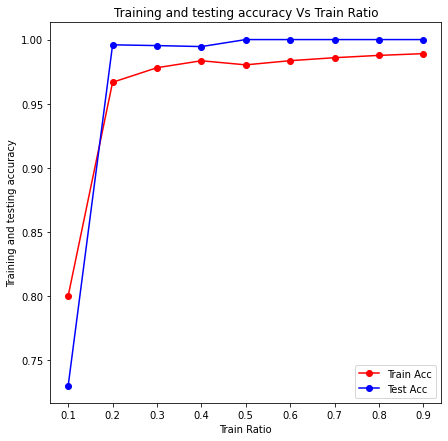
\includegraphics[width=\linewidth]{imgs/graphcovidnet_4_class_seq_accuracy.png}
      \label{fig:graphcovidnet_4_class_accuracies_seq}
    \end{subfigure}
    \begin{subfigure}{.45\textwidth}
      \centering
      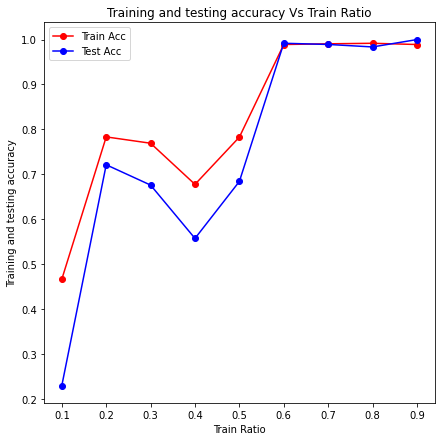
\includegraphics[width=\linewidth]{imgs/graphcovidnet_4_class_fed_accuracy.png}
      \label{fig:graphcovidnet_4_class_accuracies_fed}
    \end{subfigure}
    \caption{Comparison of centralized and federated training of GraphCovidNet on a 4-class dataset. Accuracies on the left side are from centralized training and accuracies on the right side from federated training.}
    \label{fig:graphcovidnet_4_class_accuracies}
\end{figure}

For 4-class classification the results are not perfect, but also very good. Figure \ref{fig:graphcovidnet_4_class_accuracies} shows the accuracies for all training / test splits for both our centralized and federated training. As can be seen the federated training version only achieves comparable accuracies once 60\% or more of the data is used for training purposes. This might be explained by the fact that the complete dataset does not contain a lot of images, with even less images per client when split, and that a small split in favor of training data does simply not give enough data to meaningfully train.